% ------------------------------------------------------------------------
% file `cap1TermImp-exercise-6-exercise-body.tex'
%
%     exercise of type `exercise' with id `6'
%
% generated by the `exercise' environment of the
%   `xsim' package v0.11 (2018/02/12)
% from source `cap1TermImp' on 2020/01/24 on line 54
% ------------------------------------------------------------------------
    Um estudante de física criou uma escala ($^\circ X$), comparada com a escala Celsius ele obteve o seguinte gráfico:
    \begin{figure}[ht]
        \centering
        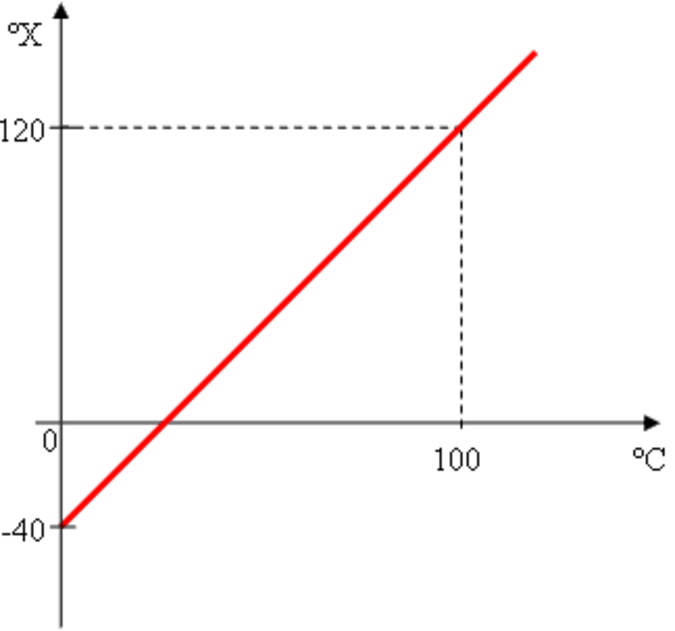
\includegraphics[scale=0.3]{graph1.pdf}
        %\caption{Exercício}
        \label{fig:graphterm1}
    \end{figure}
    \begin{enumerate}[label=\alph*),nosep]
        \item Qual a equação de conversão entre a escala $X$ e a escala Celsius?
        \item Qual a temperatura do corpo humano ($37\;^\circ C$) nesta escala?
    \end{enumerate}
